

\section{Experiments}
\label{sec:experiments}


\subsection{Discovering phonological classes}

We conducted agglomerative clustering of character embeddings in the output layer.
We found that, in all three languages, the highest-level clusters separated characters into consonants, vowels, numerals, punctuation, and various non-phonetic or rare characters.
In Figure~\ref{fig:char-clustering}, we show a clustering of German character embeddings restricted to alphabetic characters.
The top-level split partitions characters into vowels and consonants.
%Parts of the finer clustering can be phonologically motivated, e.g., the liquids r, l form a cluster
Consonant and vowel clusters each can, to a large extent, be phonologically motivated, though not along a single consistent dimensions:
(TODO describe)
%
%Within the vowel cluster: in German, vowels and their fronted umlauts together (understandable as a consequence of morphological alternations), also e/i 
%
%Clustering of consonants can partly be motivated phonologically, though not along a single consistent dimensions:
%In German, there are clusters sharing place of articulation (p/f, b/v/w, c/k/q). %, and the liquids (n/l/r) form a class 
%

\begin{figure}
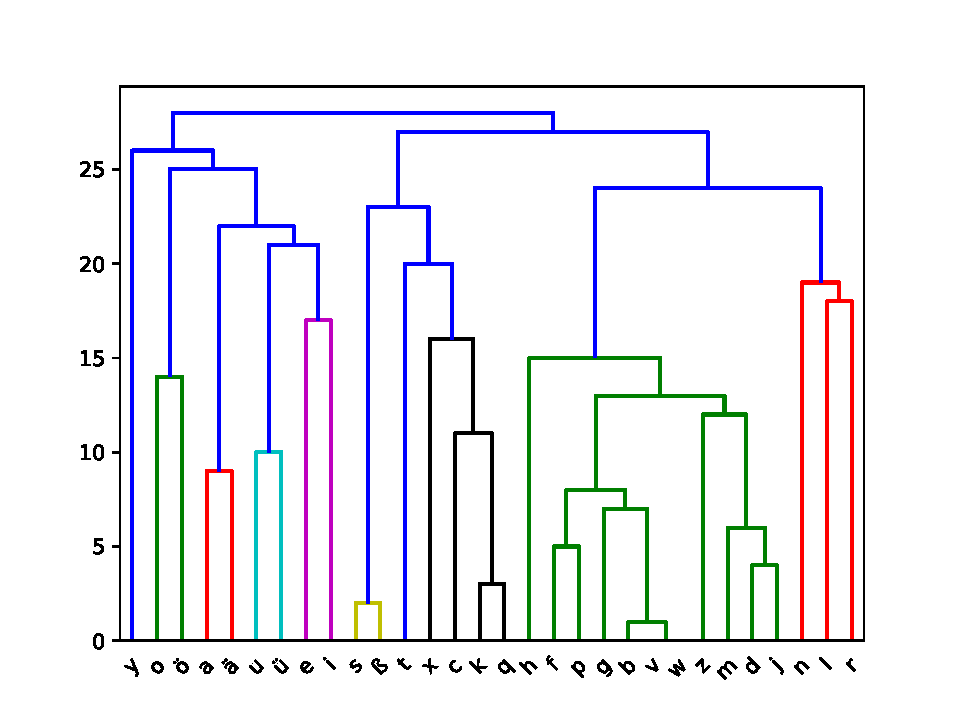
\includegraphics[width=0.50\textwidth]{figures/char-emb-clustering-output_output-phonetic-wiki-german-nospaces-bptt-910515909.pdf}
%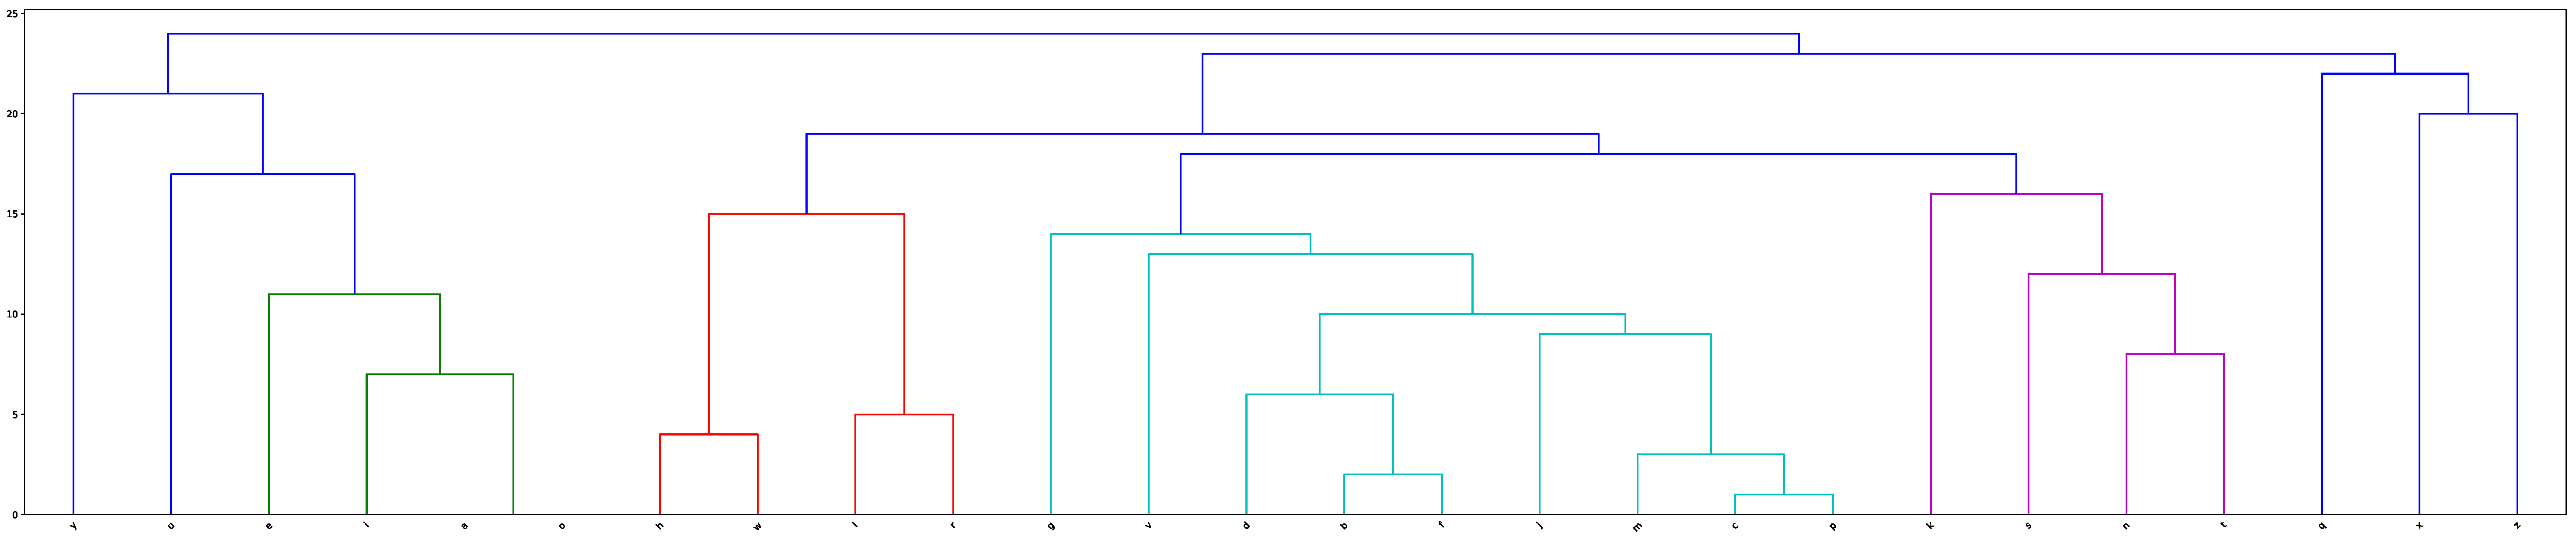
\includegraphics[width=0.48\textwidth]{figures/char-emb-clustering-output_output-phonetic-wiki-english-nospaces-bptt-282506230.pdf}
	%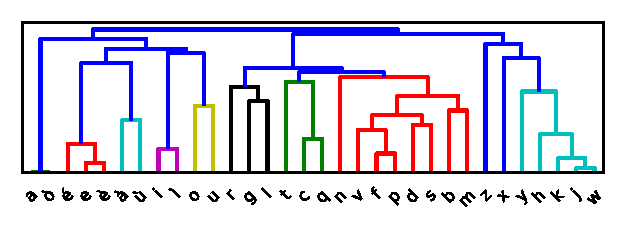
\includegraphics[width=0.48\textwidth]{figures/char-emb-clustering-output_output-phonetic-wiki-italian-nospaces-bptt-855947412.pdf}
\caption{Clustering of German character embeddings (alphabetic characters only)}\label{fig:char-clustering}
\end{figure}




\subsection{Discovering phonotactic constraints}
\label{sec:phonotactics}

Next, we study the CNLM's understanding of phonotactic constraints.
We focus on German and Italian, as they have reasonably transparent orthographies.
We construct pairs of letter bigrams (corresponding to phoneme
bigrams) beginning with the same letter, such that one is
phonotactically acceptable in the language and the other isn't, but
the independent unigram probability of the unacceptable bigram is
higher than that of the acceptable one. E.g., ``\emph{br}'' is
an acceptable Italian sequence and ``\emph{bt}'' isn't, although
\emph{``t''} is more frequent than \emph{``r''}.
For each such pair, we re-train the CNLM on a version of
the training partition from which all sequences containing either bigram have been removed.
We then look at
the likelihood the model assigns to both sequences. If the model systematically
assigns a larger probability to correct sequences, this provides evidence that it
implicitly possesses a notion of phonological categories such as
stops and sonorants, which allows it to correctly generalize from
attested (e.g., ``\emph{tr}'') sequences to unattested ones
(\emph{``br''}).

%We constructed bigram pairs where the second element was a vowel or a sonorant in the valid bigram, randomly choosing among possible vowels or sonorants if there were several.

In both languages, we constructed two groups of bigrams:
In one, the valid bigram had a vowel following a consonant; in the other, a consonant was followed by a sonorant.
In the invalid bigram, the consonant was followed by a stop or nasal.
For each onset consonant and each of the two types, we considered valid vowels or sonorants satisfying the constraint on unigram frequencies, and randomly selected one if there were several.

Results are shown in \ref{tab:phonotactics-results}.
The LSTM assigns higher probability to the valid bigrams in all but two cases.
The RNN, on the other hand, prefers the invalid bigrams, presumably because they have higher unigram probability.

This confirms that the LSTM CNLM has learnt a notion of phonological categories such as vowels and consonants, and phonotactic generalizations about them.
Note that the model makes these phonotactic generalizations entirely on the basis of distributional evidence, with no aid from perceptual or acrticulatory cues.



\begin{table}[t]
  \begin{center}
	  \begin{tabular}{p{0.2cm}p{0.2cm}|p{0.6cm}p{0.6cm}||p{0.2cm}p{0.2cm}|p{0.99cm}p{0.8cm}}
	    \multicolumn{4}{c||}{\emph{German}}   &       \multicolumn{4}{c}{\emph{Italian}}\\      \hline
	    \multicolumn{2}{c}{\emph{}}&\emph{LSTM}&\emph{RNN} & \multicolumn{2}{c}{\emph{}}&  \emph{LSTM}&\emph{RNN}\\      \hline
                     bu &  bt &  \textbf{ 4.6} &  0.22             &  bu & bd & \textbf{ 1.001} & 6e-5 \\            
                     do &  dd &  \textbf{ 1.9} &  0.05             &  du & dt & \textbf{ 1.3} & 0.008 \\             
                     fu &  ft &  \textbf{ 6.5} &  0.03             &  fu & ft & \textbf{ 30.5} & 0.01 \\             
                     po &  pt &  \textbf{ 6.4} &  0.10             &  pu & pt & \textbf{ 6.8} & 0.008 \\             
                     tu &  tt &  \textbf{ 5.4} &  0.02             &  tu & td &  0.2 & 3e-5 \\                       
		     zu &  zt &  \textbf{ 2.4} &  0.17             &  vu & vd & \textbf{ 2.0} & 2e-5 \\              \cline{1-4}
                     bl &  bd &   0.8          & 0.18              &  zu & zt & \textbf{ 55.7} & 0.01 \\              \cline{5-8} 
                     fl &  fd &  \textbf{ 2.1} & 0.82              &  br & bt & \textbf{ 1.001}  &  0.006           \\ 
                     fr &  fn &  \textbf{ 2.7} & 0.10              &  dr & dt & \textbf{ 2.5} & 0.4 \\               
                     kl &  kt &  \textbf{ 3.8} & 0.10              &  fr & ft & \textbf{ 2.9} & 0.001 \\             
                     pl &  pt &  \textbf{ 2.5} & 0.86              &  pr & pt & \textbf{ 5.0} & 0.008 \\              \hline
	    \multicolumn{2}{c|}{AM}      & \textbf{3.6} & 0.24     & 	    \multicolumn{2}{c|}{AM}   & \textbf{10.7}  & 0.041          \\
	    \multicolumn{2}{c|}{GM} & \textbf{3.0} & 0.13          & 	    \multicolumn{2}{c|}{GM}   & \textbf{3.2} & 0.0021           \\
      \hline
    \end{tabular}
  \end{center}
	\caption{\label{tab:phonotactics-results} Likelihood ratio between acceptable and unacceptable bigrams, with arithmetic (AM) and geometric (GM) means. Values $>1$ in bold.}
\end{table}

\subsection{Word segmentation}
\label{sec:segmentation}



Does the model develop an implicit notion of word?
Early work on word segmentation suggests that high uncertainty about the next character \cite{cohen-algorithm-2001, feng-accessor-2004},  low transition probabilities \cite{harris-distributional-1954, saffran-word-1996} and low mutual information \cite{sun-chinese-1998} serve as statistical cues to word segmentation.
In Figure~\ref{fig:syntax-depth}, we plot (1) entropy of the predicted distribution over the net character around word boundaries, compared to other positions, and (2) the pointwise mutual information (PMI) between left and right contexts, computed by subtracting the unconditional likelihood of the next 20 characters from their likelihood conditioned on the prior context, both computed by the CNLM on a section of the German training set.
In accordance with prior work, higher entropy and lower PMI correlate with boundaries.


\begin{figure}
	\begin{center}
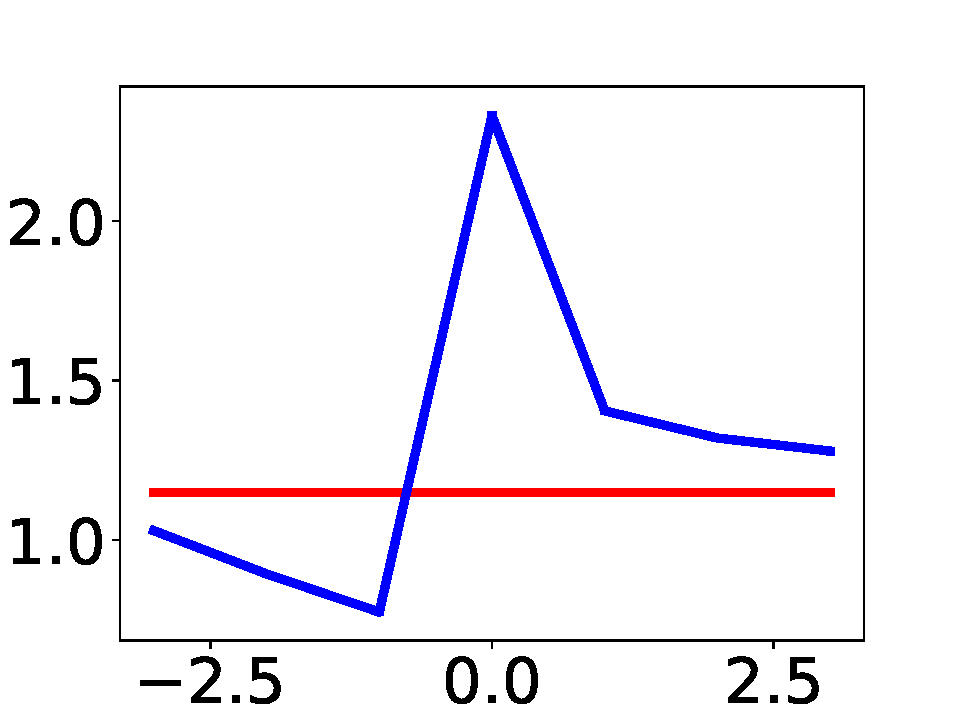
\includegraphics[width=0.22\textwidth]{figures/segmentation-profile-flattened-entropies-english-ci.pdf}
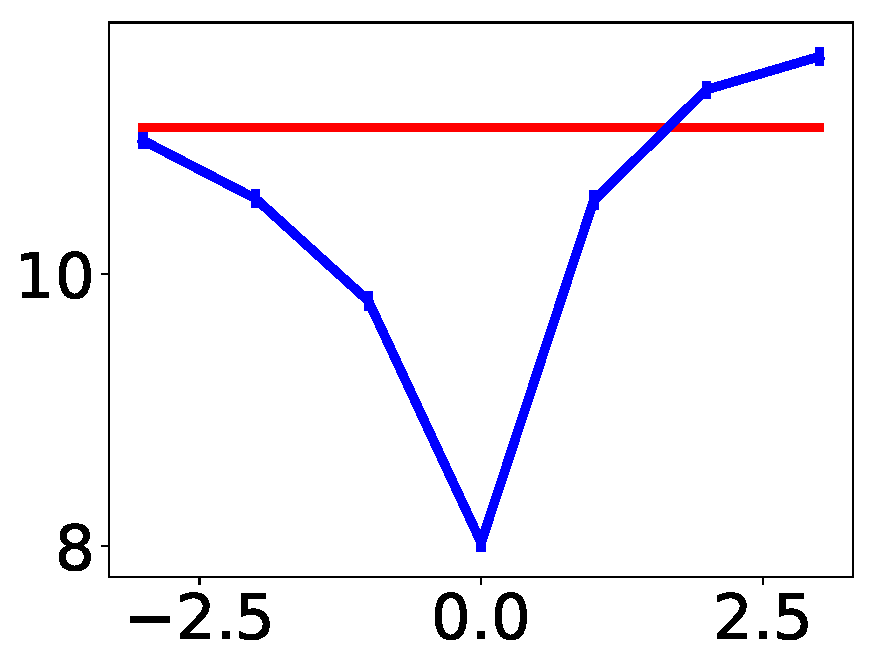
\includegraphics[width=0.22\textwidth]{figures/segmentation-profile-flattened-pmis-english-ci.pdf}
	\end{center}
	\caption{Entropy over the next character (left) and PMI between left and right contexts (right) around word boundaries (blue); the x-axis indicates position relative to a word boundary. The red line indicates the overall average of the quantity. Error bars indicate (almost imperceptible) bootstrapped 95 \% confidence intervals.
}\label{fig:boundaries-entropy}
\end{figure}


How reliable are these statistical cues, when computed by the CNLM?
We constructed a logistic regression predicting whether a character was the first one of a word or not, based on the following predictors:
(1) \emph{log-probability} of the character given prior context, (2) \emph{entropy} of the distribution over the character given prior context, (3) \emph{pmi of left and right contexts}, that is, the total likelihood of the next 20 characters, minus the unconditional likelihood estimated by starting the CNLM at the current position.
%The rationale of (3) is that it measures the pointwise mutual information, and thus the statistical association, between the subsequent characters and the prior context, which we hypothesize will be higher inside words.
%It is also the transition probability for the next characters
%(3) can also be interpreted as the result of normalizi transition probability
We collected these quantities for each position and for the preceding and following three characters.
%In total, the classifier has 21 coefficients.
We also conducted the same experiment with a character-level 8-gram model estimated on the training set, closer to the setup of earlier non-neural work.


\begin{table*}[t]
  \begin{center}
    \begin{tabular}{l|l|l|l|l}
      \multicolumn{1}{c}{}&\emph{LSTM}&\emph{RNN}&\emph{8-grams}\\
      \hline
      English & 65.83/60.37/62.98 &   63.26/59.81/61.49 & 55.73/51.0/53.26    \\ % \ldots{}/\ldots{}/\ldots & \ldots{}/\ldots{}/\ldots & \ldots{}/\ldots{}/\ldots &\ldots{}/\ldots{}/\ldots\\
      German &  57.012/52.505/54.67 &  53.2/49.26/51.15 & 42.89/36.28/39.31   \\ %   \ldots{}/\ldots{}/\ldots & \ldots{}/\ldots{}/\ldots & \ldots{}/\ldots{}/\ldots &\ldots{}/\ldots{}/\ldots\\
      Italian &  63.59/56.95/60.09 & 62.47/57.5/59.89  & 48.41/39.62/43.57    \\ % \ldots{}/\ldots{}/\ldots & \ldots{}/\ldots{}/\ldots & \ldots{}/\ldots{}/\ldots &\ldots{}/\ldots{}/\ldots\\
    \end{tabular}
  \end{center}
  \caption{\label{tab:segmentation-results} Precision recall, and F1 on word segmentation.}
\end{table*}

%PMI alone 
%P 30.56 R 20.61 F 24.61 German
%P 32.19 R 20.89 F 25.34 Italian
%P 39.37 R 29.45 F 33.69 English
%Surprisal alone
%P 28.04 R 18.64 F 22.4 German
%P 28.76 R 18.31 F 22.38 Italian
%P 33.65 R 24.1 F 28.08 English
%Entropy alone
%P 50.88 R 45.57 F 48.08 German
%P 58.44 R 52.09 F 55.08 Italian
%P 59.85 R 53.75 F 56.63 English


For each language model and language, we compute how many of the extracted tokens were correct (precision) and how many of the actual tokens were found by the classifier (recall), together with F1.
The goal of this experiment is not to construct a new word segmentation system, but to evaluate how strongly the CNLM's probabilities are indicative of word boundaries.

Results are shown in Figure~\ref{tab:segmentation-results}, showing that the CNLM-based classifiers robustly segment more than half of the tokens correctly, and do considerably better than the character 8-gram model.
Ablation shows that entropy is most predictive, reaching an F1 of 56.63 (English), 48.08 (German), 55.08 (Italian) alone.
Surprisal reaches 28.08 (English), 22.4 (German), 22.38 (Italian); PMI reaches 33.69 (English), 24.61 (German), 25.34 (Italian).
%Setting N to other values shows that larger values of N increase performance (N =10: 62.45, N=20: 63.24).

How does the LSTM CNLM compare to unsupervised word segmentation models?
We compare to the Bayesian bigram model of \cite{goldwater-bayesian-2009}, an elegant model using a hierarchical Dirichlet process.
Running Bayesian methods on the Wikipedia dumps is computationally infeasible; thus we also created a CNLM on the Brent corpus \cite{brent-efficient-1999} of child-directed speech.
We used 90 \% to train our language model, 5 \% to fit the logistic regression, and 5 \% to evaluate word segmentation.
(This compares with the Bayesian models that train and evaluate on the full dataset, but incorporate no word boundary information in their training signal).

\begin{table*}[t]
  \begin{center}
    \begin{tabular}{ll|l|l|l|l}
      \multicolumn{2}{c|}{}&Tokens & Lexical & Boundaries\\      \hline
	    \multirow{4}{*}{CNLM} & Full model & 0.75/0.76/0.75 & 0.41/0.61/0.49 & 0.91/0.90/0.90 \\
	    &     log-probability & 0.510/0.453/0.480 & 0.488/0.195/0.279 & 0.805/0.716/0.758 \\
	    &     entropy & 0.504/0.533/0.518 & 0.520/0.211/0.300 & 0.790/0.747/0.768\\
	    &     PMI & 0.708/0.729/0.718 & 0.576/0.346/0.432 &0.899/0.873/0.886  \\ \hline
	    \multicolumn{2}{c|}{\citet{goldwater-bayesian-2009}} & 0.752/0.696/0.723 & 0.635/0.552/0.591 & 0.903/0.808/0.852
    \end{tabular}
  \end{center}
	\caption{\label{tab:segmentation-results-brent} Word segmentation results on the Brent corpus for our model, for the three individual predictors, and the Bayesian model of \cite{goldwater-bayesian-2009}. Following \cite{goldwater-bayesian-2009}, we evaluate on the level of tokens, the lexicon of induced word types, and boundaries.}
\end{table*}

Results in Table~\ref{tab:segmentation-results-brent} show that the performance is broadly comparable to that of a sophisticated Bayesian segmentation method.
This suggests that statistical properties as modeled by the CNLM provide reliable cues to word boundaries.\footnote{We also created a logistic regression on hidden states, obtaining accuracy over 90 \% in classifying word boundaries on unseen words, outperforming an n-gram-count baseline. This suggests that the model internally tracks word boundaries.}
In contrast to the Wikipedia experiments, PMI emerges as the most important predictor on this dataset.

Unlike our method, the Bayesian method is fully unsupervised, but it has a built-in bias towards a discrete lexicon with a power-law frequency distribution.
Note that, unlike supervised word segmentation methods, our classifier does not have access to the character strings directly; instead, it evaluates how strongly quantities computed by the CNLM \emph{correlate} with word boundaries.



Looking at the main errors made by our English CNLM is instructive. We
consider first the 30 most common undersegmentations in the test set
(that is, cases in which the model failed to split two or more
words). About half (16) of them are common function word sequences
that could indeed easily be re-analyzed as single words (e.g.,
\emph{more than}, \emph{as well as}, \emph{such as}). Of the remaining
cases, 8 follow the \emph{N of} pattern, where \emph{N} is a
(typically relational) noun commonly occurring in this construction
(\emph{member of}, \emph{end of}, \emph{part of}\ldots). There are 3
fixed multi-word expressions (\emph{New York}, \emph{United States}
and \emph{high school}). Finally, it's reasonable to treat \emph{based
  on}, \emph{known as} and \emph{according to} as lexicalized
connectives, especially in the Wikipedia text the model was trained
upon.

The picture is a bit murkier but still fairly linguistically grounded
for the 30 most common oversegmentation errors (that is, the character
fragments that are wrongly segmented from inside the largest number of
distinct words).\footnote{We ignore here single-letter segmentations,
  that would otherwise account for one third of the most-frequent
  set.}  More than half (17) are common affixes (prefixes such as
\emph{re} and \emph{de} or suffixes such as \emph{ing} and
\emph{ly}). The remaining cases include 3 strings identical to frequent
function words wrongly carved out of longer words (\emph{the},
\emph{to} and \emph{on}, although the model might be treating the
latter as a pseudo-suffix in forms such as \emph{Peterson} and
\emph{Creighton}). Further, the strings \emph{land} and \emph{man} are not
unreasonably segmented out of compounds. It's hard, on the other hand,
to find a linguistically sound motivation for the 8 remaining top
oversegmentations (\emph{la, le, ma, na, ra, ro, se, ta}).

We hypothesized that similar statistical correlates exist for hierarchical syntactic structure.
We created constituency trees for the German validation set using the Berkeley Parser~\ref{petrov2007improved}.
For each character in the data, we counted its hierarchical distance from the preceding character, operationalized as the number of intervening closing and opening brackets.
This number is zero if and only if both characters belong to the same word.

Figure~\ref{fig:syntax-depth} plots PMI by hierarchical distance, for all distances for which at least 1000 datapoints occurred in the dataset.
The plot shows that longer hierarchical distance between neighboring characters corresponds to lower average MI, generalizing the finding for word boundaries.
This illustrates how it is useful for segmentation knowledge to be implicit, as the model ``knows'' about different kinds of boundaries in a continuous manner.

\begin{figure}
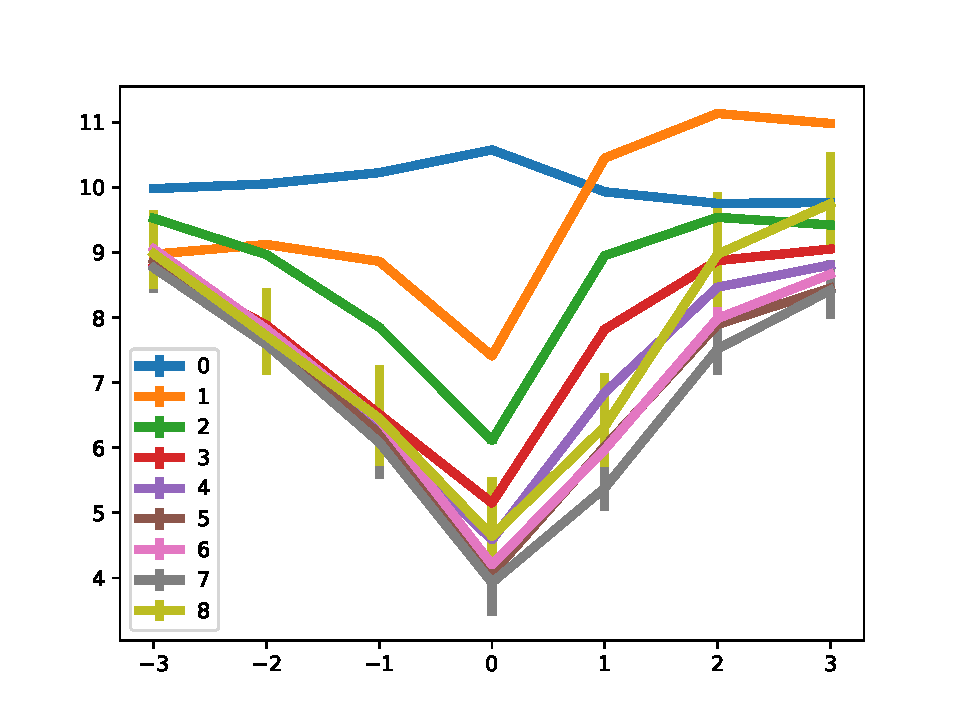
\includegraphics[width=0.48\textwidth]{figures/segmentation-profile-pmis-german-all-heights-ci.pdf}
\caption{PMI between left and right contexts, estimated by the CNLM, by syntactic hierarchical distance between subsequent characters, and bootstrapped 95 \% confidence intervals.}\label{fig:syntax-depth}
\end{figure}



%687112
%73757
%46716
%22847
%7896
%2587
%827
%234
%80




\subsection{Discovering morphological categories}
\label{sec:categories}

Does the CNLM discover morphological categories?
Note that these are lexical
properties, probed in a model that has no explicit notion of word.
We again focus on German and Italian given massive morphosyntactic ambiguity
and impoverished morphology of English.

\paragraph{Word classes (nouns vs.~verbs)}

Does the model implicitly encode word classes?
We sampled 500 verbs and 500 nouns from the training set, each with the requirement that they end in -\emph{en} (German) or -\emph{re} (Italian), and that they did not occur both as nouns and verbs.
We did this since these final syllables are common among both verbs and nouns, setting the bar higher for methods relying on surface cues.
We then recorded the hidden states of the CNLM after reading each of these words, without context.
We randomly selected N=20 training examples, balanced between the two POS classes, to create a logistic classifier distinguishing nouns and verbs from the hidden states of the LSTMs, and tested on the remaining examples.
We repeated this experiment 100 times to control for variation between the random train-test splits.

As a baseline, we created a character-level LSTM autoencoder which was been trained to reconstruct individual words in isolation.
We expect that the hidden state of the autoencoder encodes orthographic features relevant for the languages.
We further considered word embeddings from the output layer of the word-based language model, removing OOV words from the evaluation of this model.

Results are shown in Table~\ref{tab:pos-results}.
Across the board, models based on language models outperform those constructed from autoencoders, showing  that model has learned categories based on broader distributional evidence, not just typical strings cueing nouns and verbs.


We then varied N from 2 to 100.
Resulting accuracies for German are shown in Figure~\ref{fig:pos-induction}; they confirm that the CNLM-based encodings distinguish the categories well for small training sets, while the autoencoder does not catch up even with 100 training examples per category.
Results were qualitatively identical in Italian.

\begin{table}[t]
  \begin{center}
    \begin{tabular}{l|l|l}
   &\emph{German}&\emph{Italian}\\
      \hline
      LSTM & 89.0 & 94.0 \\
      RNN & 82.0 & 91.9 \\
      Autoencoder & 65.1 & 82.8 \\
      WordNLM & 97.4 & 96.0 \\
    \end{tabular}
  \end{center}
  \caption{\label{tab:pos-results} POS accuracy (20 training examples per category)}
\end{table}


\begin{figure}
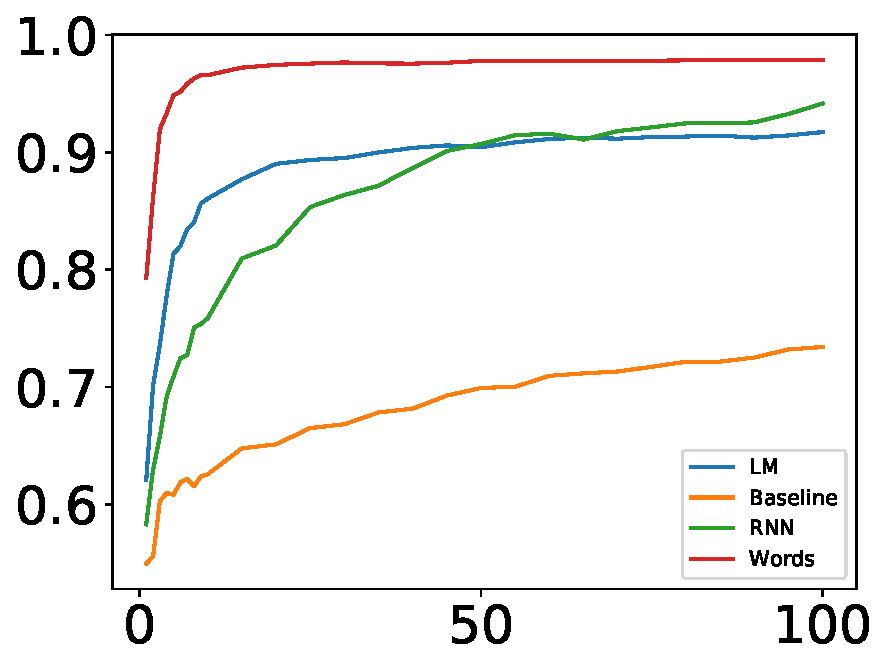
\includegraphics[width=0.48\textwidth]{figures/german_pos_nouns_verbs.pdf}
	\caption{POS accuracy as a function of training examples.}\label{fig:pos-induction}
\end{figure}





\paragraph{Number}
Does the hidden state of the CNLM store an abstract notion of
number?
German nouns can be binned in different classes depending on
the morpheme or morphological process they use to form the plural. We
train a number classifier on a subset of these classes, test on the
others: if model generalizes correctly, it means that it knows about
number independently of its surface expression.

We extracted plural nouns from the German Universal Dependencies treebank \cite{de2006generating,mcdonald2013universal}.
We selected plurals formed with -\emph{n}, -\emph{s}, or -\emph{e} suffixation to train the classifier, and tested on plurals formed with -\emph{r} suffixation or vowel change (\emph{umlaut}).

For the training set, we randomly selected 30 singulars and 30 plurals from each of the training classes.
As plural suffixes make words longer, we used rejection sampling from a single distribution over lengths to ensure that the lengths of the singular and plural examples were approximately matched.
For the test set, we selected all plurals with -\emph{r} suffix or vowel change together with their respective singulars.

As before, we consider an autoencoder and embeddings from a word-level language model as baselines.

To control for the impact of random selection of training samples, we repeated this 200 times and averaged the resulting accuracies on number classification.
Results are summarized in Table \ref{tab:number-results}.


\begin{table}[t]
  \begin{center}
    \begin{tabular}{l|l|l|l}
      &\emph{-n, -s, -e}&\emph{-r}&\emph{Umlaut}\\      \hline
      LSTM& 82.1/68.0/83.7  & \textbf{88.2} & 52.8 \\
      RNN& 77.6/60.0/73.4 & 81.3 & 53.3\\
      Autoencoder& 73.2/54.5/64.4 & 73.8 & 59.2\\
      WordNLM& \textbf{97.1/97.9/98.5} & 86.6 & \textbf{96.7}  \\ % when including OOVs: 81.0/83.8/81.5 & 72.9 & 77.6\\
    \end{tabular}
  \end{center}
  \caption{\label{tab:number-results} Accuracy for classifying number. The random baseline is 50 \%.}
\end{table}

%python char-lm-ud-stationary-separate-bidir-with-spaces-probe-baseline-prediction-wiki-plurals-2-tests-RNN.py  --batchSize 256 --char_dropout_prob 0.01 --char_embedding_size 50 --char_noise_prob 0.0 --hidden_dim 2048 --language german --layer_num 2 --learning_rate 0.1 --nonlinearity tanh --load-from wiki-german-nospaces-bptt-rnn-237671415 --sequence_length 30 --weight_dropout_hidden 0.0 --weight_dropout_in 0.0
%python char-lm-ud-stationary-separate-bidir-with-spaces-probe-baseline-prediction-wiki-plurals-2-tests-words.py  --language german --batchSize 128 --char_embedding_size 200 --hidden_dim 1024 --layer_num 2 --weight_dropout_in 0.1 --weight_dropout_hidden 0.35 --char_dropout_prob 0.0 --char_noise_prob 0.01 --learning_rate 0.2 --load-from wiki-german-nospaces-bptt-words-966024846


The classifier based on word embeddings is overall the most successful, confirming that word embeddings encode number reliably.
Encodings from the CNLM outperform the autoencoder on plurals formed with suffixes, indicating some generalization to unseen plurals beyond orthographic cues.
In the case of -\emph{r} plurals, the CNLM LSTM generalizes better than the word NLM.
In contrast, almost no generalization to plurals formed by vowel change is found, suggesting that the CNLM does not consistently encode noun number in a fully generalizable way -- at least not in a way accessible to a logistic classifier.


\subsection{Capturing syntactic dependencies}
\label{sec:dependencies}

Despite not having pre-defined information about words and morphemes, is the model able to capture non-adjacent syntactic dependencies?
In particular, is it able to do so when dependencies cross one or more words, and thus cannot be reduced to surface n-gram counts?
Note that, for a CNLM, dependencies across even a single word are often already long-distance. % even \emph{``\textbf{la} bell\textbf{a}''} is long distance.
We again focus on German and Italian due to the richness of inflectional morphology in these languages.
Constructions will be language-specific, so we discuss the languages separately. %German and Italian separately (not much in English).

%As usual, specifics of training etc that depart from general setup.




\paragraph{German} We consider 4 constructions:
\begin{inparaenum}[i)]
\item article-noun gender agreement, possibly with material in the middle,
\item determiner-noun case concord, again with material in the middle,
\item preposition case sub-categorization, with material in the middle.
\end{inparaenum}


\paragraph{German Gender Agreement}
Each German noun belongs to one of three genders (masculine, feminine, neuter), which are morphologically marked on the article.
As the article and the noun can be separated by adjectives and adverbs, we can probe not only the CNLM's knowledge of nouns' genders, but also its ability to model gender agreement across distances.
We create stimuli of the form
\begin{enumerate}[label={(\arabic*)}]
	\item \begin{tabular}[t]{lllllll}
	\{\underline{der}, die, das\}& sehr& rote& Baum \\
	article & adverb & adjective & noun \\
	the & very & red & tree
\end{tabular}
\end{enumerate}
where the correct nominative singular article (\emph{der}, in this case) matches the gender of the noun.
We then run the CNLM on the three versions of this phrase (removing whitespace) and record the probabilities it assigns to them.
If it systematically assigns the highest probability to the correct version, we have evidence that the CNLM has learnt the association between the noun and the form of the article.
To indicate that there are word boundaries at the beginning and end of the phrase (e.g., \emph{der} could also be the end of another word), we add a full stop before and after the stimulus when running the CNLM.

%  \cite{de2006generating,mcdonald2013universal}
We select all nominative singular nouns from the German Universal Dependencies treebank. %, and all adjectives from the training set.
We construct four conditions varying the number of adverbs and adjectives between the article and the noun.
We first consider stimuli where no material intervenes.\footnote{Due to syncretism in the article paradigm, there sometimes is ambiguity in the choice of the correct article if the noun's morphology does not uniquely indicate that it is nominative singular. As this affects all feminine nouns, we did not remove such cases. Importantly, this issue is solved as soon as an adjective is present, as their form uniquely indicates that the phrase is nominative singular.}
In the second condition, an adjective with the correct (nominative singular) case ending, randomly selected from the training corpus, is added.
Crucially, the ending of the adjective does not reveal the gender of the noun.
In the third and fourth condition, one (\emph{sehr}) or two adverbs (\emph{sehr extrem}) intervened between the article and the adjective.
These also do not reveal the noun's gender.

Besides the CNLMs and the word-level language model, we also construct an n-gram baseline that chooses the version that occurs most frequently in the training data, and randomly chooses in case of a tie (e.g., if no version was observed).
When running the word-level model, we excluded nouns that were out of vocabulary.

In Figure~\ref{fig:gender}, we report accuracy for nouns from each of the three genders, and the average over the genders.
Across genders and conditions, the word-level LSTM tends to perform best, followed by the CNLM.
While the n-gram baseline performs similarly to the CNLM when there is no intervening material, accuracy drops to the random baseline (0.33) in the presence of an adjective.
%This can partly be attributed to our choice to choose the adjective randomly from the vocabulary.
Note that this would not be mitigated by models that include interpolation with or backoff to lower-order n-grams, as the relevant gender information is present only on the first and last word of each stimulus.
This contrast shows that, while the association between articles and nouns can be learnt from simple corpus statistics, the CNLM has some capability to preserve the relevant information across more than a dozen timesteps.
The RNN CNLM is weaker across conditions, and its accuracy drops to random as more intervening material is present.

The exclusion of OOVs and thus limiting experiments on word-level models to frequent words might create an unfair advantage; running the CNLM only on those stimuli given to the word-level model results in slightly better accuracies but the same pattern of results.

\begin{figure*}
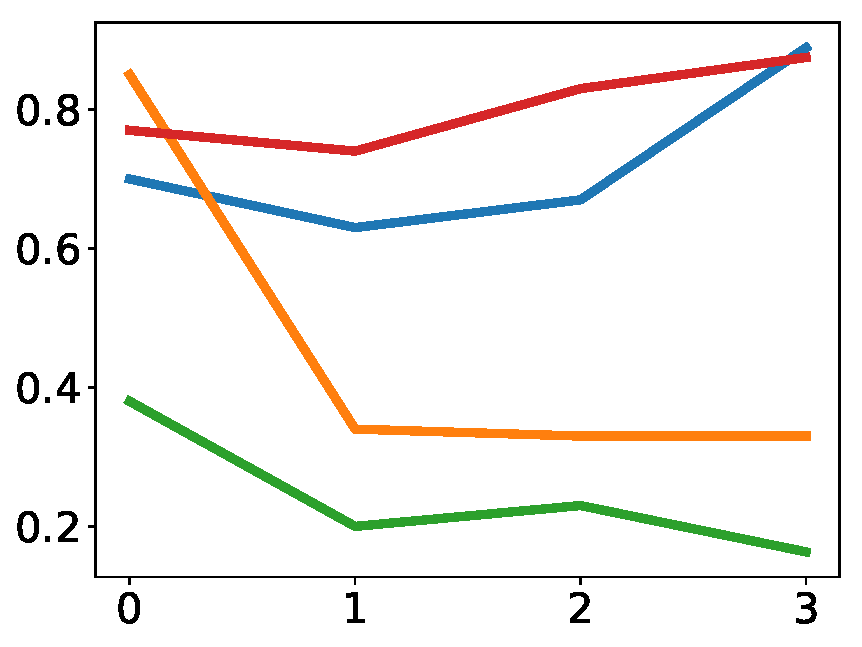
\includegraphics[width=0.24\textwidth]{figures/german-gender-m.pdf}
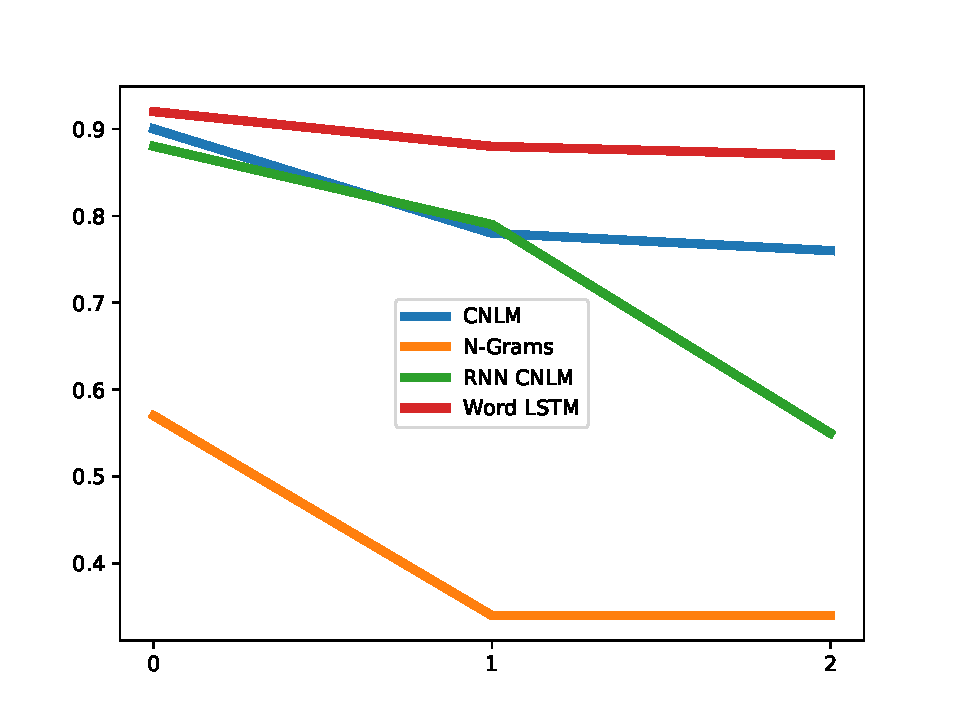
\includegraphics[width=0.24\textwidth]{figures/german-gender-f.pdf}
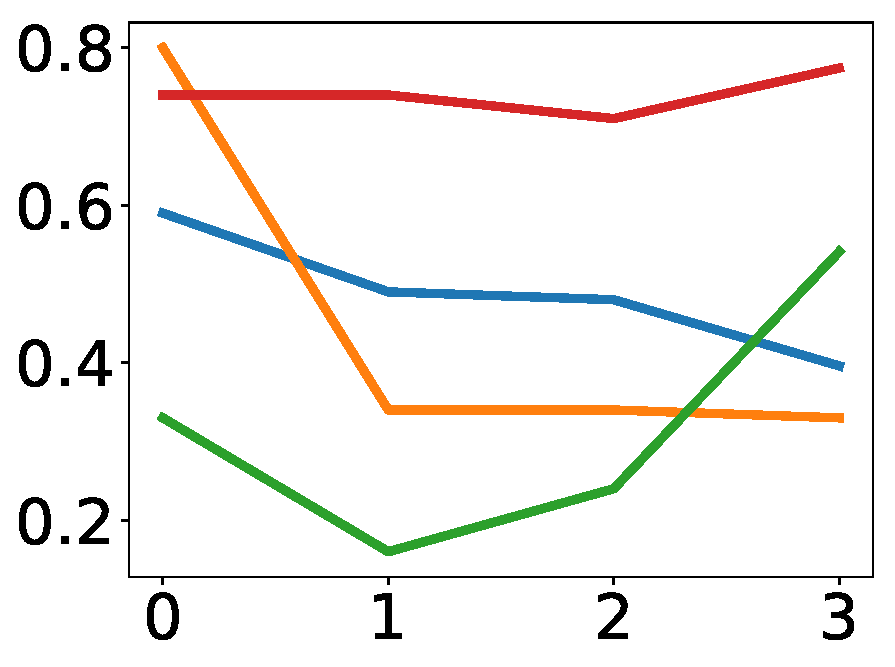
\includegraphics[width=0.24\textwidth]{figures/german-gender-n.pdf}
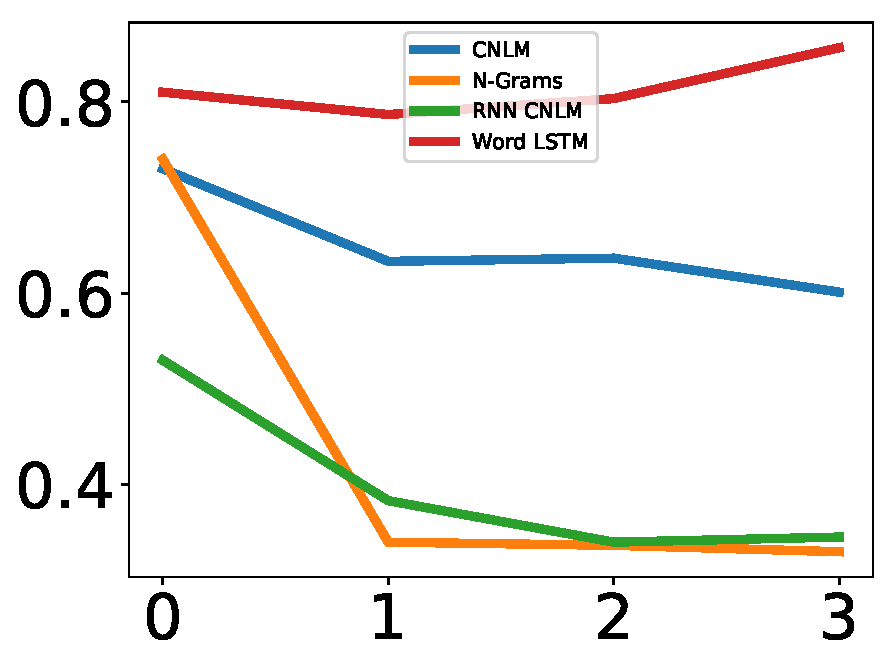
\includegraphics[width=0.24\textwidth]{figures/german-gender-total.pdf}

\centering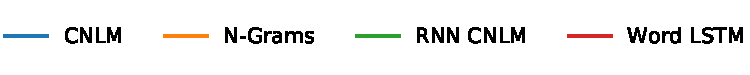
\includegraphics[width=0.5\textwidth]{figures/german-legend.pdf}
\caption{Accuracy on the Gender Agreement task as a function of the number of intervening elements, for masculine, feminine, and neuter nouns, and across all three classes.}\label{fig:gender}
\end{figure*}


\paragraph{Case Agreement}
Here we test the model's knowledge of case agreement between articles and nouns.
We selected the two determiners \emph{dem} and \emph{des}, which unambigously indicate dative and genitive case, respectively, for masculine and neuter nouns.
We also selected all nouns of the appropriate genders that unambigously mark these two cases.
We selected noun lemmas from the Universal Dependencies treebank, and extracted morphological paradigms for Wiktionary to obtain case-marked forms.
We created four conditions, varying the amount of intervening material, as in the gender agreement experiment.

Results are shown in Figure~\ref{fig:case}.
Again, the Word LSTM has the strongest overall performance, but the CNLM is competitive as more elements intervene. Accuracy stays well above 80 \% even as three words intervene.
The n-gram model performs well if there is no intervening material, and at chance otherwise.
Accuracy of the RNN CNLM remains above chance for one or two intervening elements, but drops considerably.

Considering the results for the dative and genitive separately, accuracy slightly increases in the dative case and decreases in the genitive case.
This can be attributed to the higher baseline frequency of dative in German, suggesting that both word- and character-based networks are impacted by unigram frequencies as more words intervene.
This effect is far more pronounced for the RNN CNLM, explaining its overall decrease to chance level.
Again, restricting to words that are in the word-level vocabulary did not change the pattern of results.
\begin{figure}
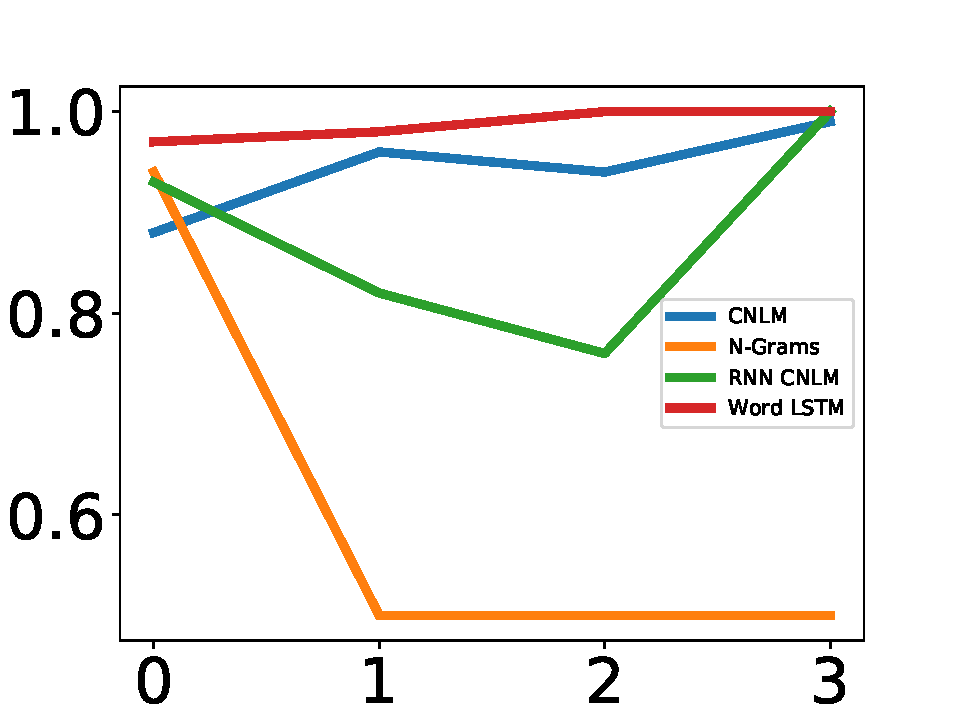
\includegraphics[width=0.23\textwidth]{figures/german-case-Dative.pdf}
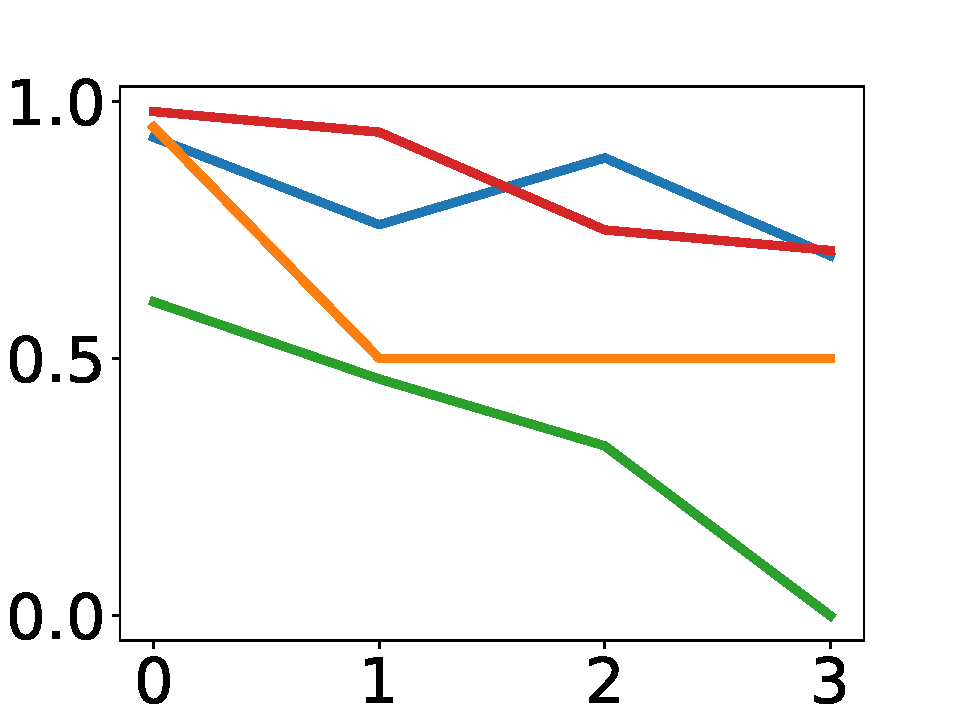
\includegraphics[width=0.23\textwidth]{figures/german-case-Genitive.pdf} \\

\centering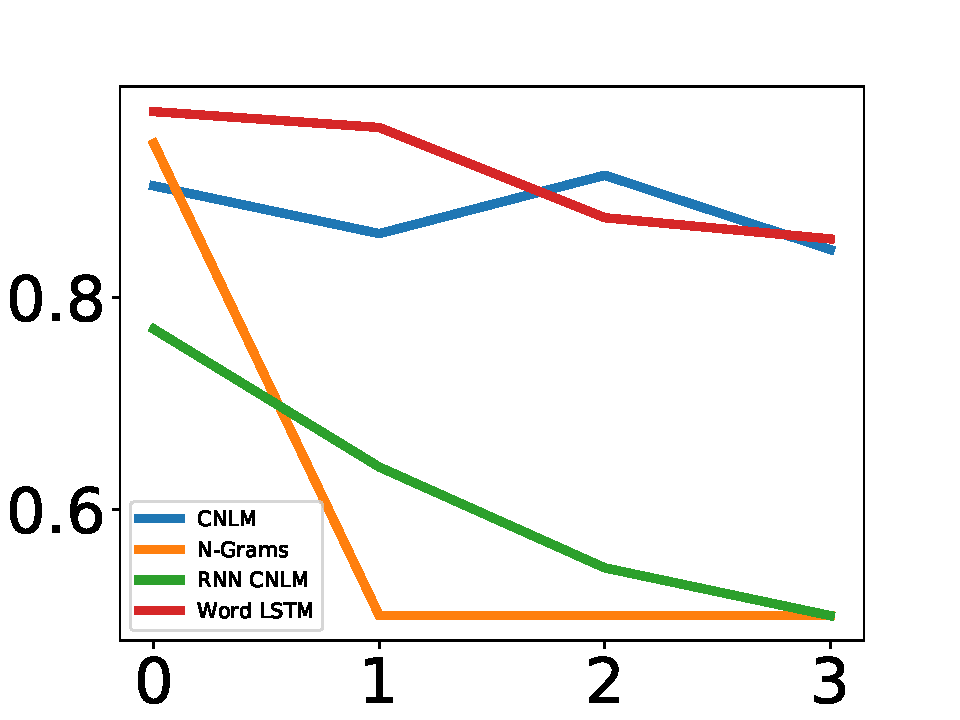
\includegraphics[width=0.24\textwidth]{figures/german-case-total.pdf}

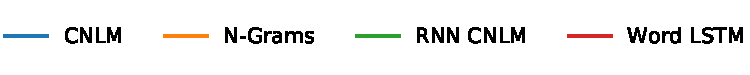
\includegraphics[width=0.5\textwidth]{figures/german-legend.pdf}
	\caption{Accuracy on the Case Agreement task as a function of the number of intervening elements, for dative and genitive phrases (top), and across the two cases (bottom).}\label{fig:case}
\end{figure}

\paragraph{Case Subcategorization}
German verbs and prepositions lexically specify the case appropriate to their objects (mostly dative or accusative).
We probe the CNLM's knowledge of such generalizations using the preposition \textit{mit} `with', which selects for a dative object.

To focus on knowledge of subcategorization (as opposed to inflectional paradigms), we construct objects whose head noun is a nominalized adjective, whose inflection is very regular.
We take all adjectives that occur at least 100 times in the training data, excluding those that end in -\emph{r}, as these often reflected lemmatization problems.

We then selected all sentences containing a `mit' prepositional phrase in the German Universal Dependencies treebank, subject to the constraints that (1) the object is not a pronoun (such objects often are relative or interrogative pronouns and cannot be replaced with a nominal object without sacrificing grammaticality), and (2) the object is a continuous phrase.
For each sentence, we remove the prepositional phrase and replace it by a phrase of the form
\begin{enumerate}[label={(\arabic*)}]
	\item \begin{tabular}[t]{lllllll}
	mit & der & sehr& \{rote, \underline{roten}\} \\
	prep & article  & adverb & adjective \\
	with & the & very  & red one 
\end{tabular}
\end{enumerate}
where only the \emph{-en} version of the adjective is compatible with the case requirement of the preposition.
Note that this correct version is longer than the incorrect one; this ensures that the bias for shorter sequences works against the model.
We construct three conditions by varying the presence and number of adverbs (\emph{sehr} `very', \emph{sehr extrem} `very extremely', \emph{sehr extrem unglaublich} `very extremely incredibly').
As a control for baseline probabilities of the two versions of the adjective, we also created control stimuli where all words up to the preposition were removed, and computed accuracy on these stimuli.
If accuracy is lower on these stimuli than on the full stimuli, we can conclude that baseline probabilities of the two adjective forms cannot explain success on the task.

For the n-gram count model, we only counted the occurrences of the prepositional phrase, omitting the environment.

\begin{figure}
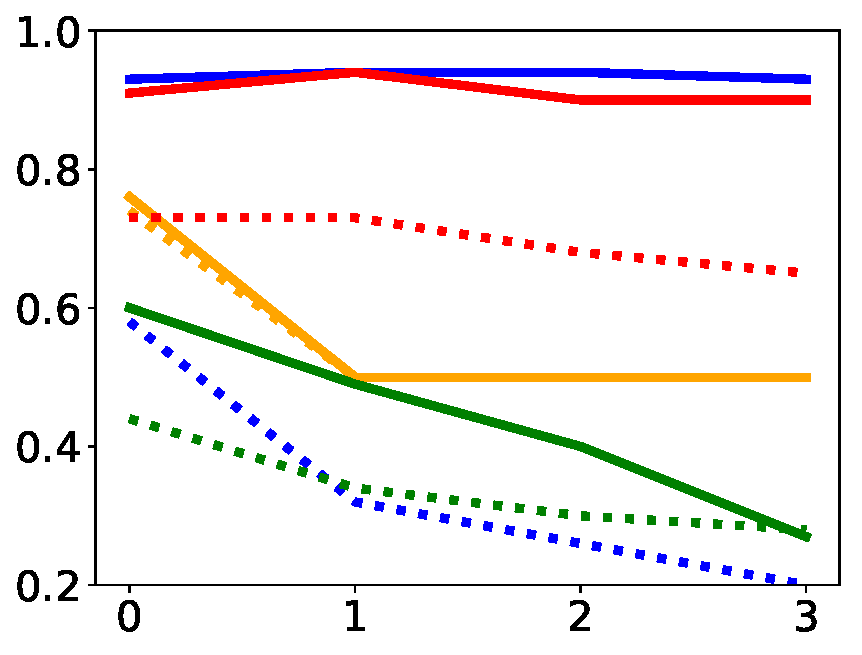
\includegraphics[width=0.48\textwidth]{figures/german-prep-with-control.pdf}

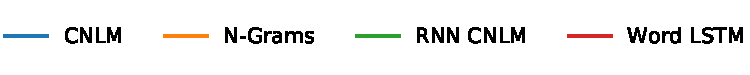
\includegraphics[width=0.48\textwidth]{figures/german-legend.pdf}
\caption{Accuracy on the Subcategorization task as a function of the number of intervening elements. For eavh model, the dashed line indicates accuracy on the control stimuli that do not contain the preposition.}\label{fig:prep}
\end{figure}

Results are shown in Figure~\ref{fig:prep}.
All models except the one based on n-gram counts outperform the accuracy achieved on the control stimuli that did not include the preposition, showing that their performance cannot be attributed to baseline frequencies of the adjective forms, and that they take the preposition into account when choosing the adjective form.
The CNLM slightly outperforms the word-level language model, even though the CNLM has a harder task as it is not limited to the 50,000 most frequent words.
Neither model shows accuracy decay as the number of adverbs increases.
As before, the n-gram model drops to chance as adverbs intervene, while the RNN CNLM starts with low accuracy that decays below chance.



%Results are shown in Table~\ref{tab:ital-agr-results}.
%The word LSTM shows the highest overall performance, closely followed by the LSTM CNLM.
%The RNN performs well on adjective gender, and considerably worse than the CNLM on the other tasks.
%For the CNLMs, the most challenging task was article-noun gender agreement.
%Discussion case-by-case, including how we control for n-gram frequency
%and length.
%Results table with a row for each pattern and a column for each model.


\paragraph{Italian} We consider further constructions from Italian that confirm the results we got in German.
Here, we focus on a  subset of Italian morphology where gender and number are explicitly and systematically
encoded while allowing for tightly controlled comparison of
same-length strings, limited to stimuli unseen in the training corpus.
\begin{inparaenum}[i)]
\item article-noun gender agreement with material in the middle,
\item article-adjective gender agreement, with an adverb in the middle,
\item article-adjective number agreement, with an adverb in the middle.
\end{inparaenum}

\paragraph{Article-Noun Gender Agreement}
%(1) eadj-aonoun:

Similar to German, Italian articles agree with the noun in gender; however, while gender is often unpredictable in German, Italian has a productive system of forming masculine and feminine versions of nouns that differ in the final vowel (-\emph{o} for masculine, -\emph{a} for feminine).
We construct stimuli of the form:
\begin{enumerate}[label={(\arabic*)}]
	\item 
		\begin{tabular}[t]{lllllll}
	a. & \{\underline{il}, la\} & congeniale & candidato \\
   &  the & congenial & candidate (m.) \\
	& \multicolumn{4}{l}{`The congenial male candidate.'} \\
	b. & \{il, \underline{la}\} & congeniale & candidata \\
    &the & congenial & candidate (f.) \\
	& \multicolumn{4}{l}{`The congenial female candidate.'} \\
\end{tabular}
\end{enumerate}

Note that the intervening adjective, ending in -\emph{e}, does not reveal the noun's gender, increasing the distance across which gender information has to be transported.

We constructed these stimuli such that none of the adjective-noun pairs appear in the training data, and all single words appear at least 100 times.
Further, the nouns in -\emph{a} and  -\emph{o} have reasonably balanced frequency (neither form is twice more frequent than the other), or they are both frequent (appear at least 500 times)
As the prenominal adjectives are somewhat marked in Italian, we  we considered only -e adjectives that occur at least with 10 different nouns in the prenominal position.

Results are shown in the first line in Table~\ref{tab:ital-agr-results}.
The word LSTM shows the strongest performance, closely followd by the LSTM CNLM.
Even the RNN CNLM performs strongly above chance.

\paragraph{Article-Adjective Gender Agreement}
We then created an experiment where an adverb intervened between an article and an adjective, both of which were marked for gender:
\begin{enumerate}[label={(\arabic*)}]
	\item 
		\begin{tabular}[t]{lllllll}
	a. & il & meno & \{ \underline{alieno}, aliena \} \\
   &  the & less & alien one  \\
	b. & la & meno & \{ alieno, \underline{aliena} \} \\
    &the & less & alien one \\
\end{tabular}
\end{enumerate}
where we used the adverbs \emph{pi{\`u}} `more', \emph{meno} `less', \emph{tanto} `so much'.
We considered only adjectives that occurred 1K times in the training corpus, as this is the most common kind of adjective in Italian.
We excluded all cases in which the adverb-adjective combination occurred in the training corpus, in either feminine or masculine form.


% /checkpoint/mbaroni/char-rnn-exchange/candidate_adv_aoadj_testset.txt

Results are shown in the second line in Table~\ref{tab:ital-agr-results}; all three models perform almost perfectly.

\begin{table}[t]
  \begin{center}
    \begin{tabular}{l|ll|ll|ll}
	    & \multicolumn{4}{c|}{CNLM} & \multicolumn{2}{c}{\multirow{2}{*}{Word LSTM}}\\
	    &\multicolumn{2}{c|}{\emph{LSTM}}&\multicolumn{2}{c|}{\emph{RNN}} &\\ \hline
% eadj-aonoun
	    Noun Gender & 97&90  & 84&73 & 99&96 \\
%      adv-aoadj
	    Adj. Gender & 99&100 & 100&97 & 98&100 \\
% adv-aeadj
	    Adj. Number & 99&99 & 99&70 & 100&100 \\
    \end{tabular}
  \end{center}
	\caption{\label{tab:ital-agr-results} Results for morphosyntactic tests in Italian. For each model and test, we show accuracy on the two types of stimuli (masculine/feminine for gender, singular/plural for number).}
\end{table}

\paragraph{Article-Adjective Number Agreement}
We then constructed a version of the last test that probed number agreement instead of gender agreement; number marking is similarly very systematic in Italian.
Stimuli had the form
\begin{enumerate}[label={(\arabic*)}]
	\item 
\begin{tabular}[t]{lllllll}
	a. & la & meno & \{ \underline{aliena}, aliene \} \\
   &  the & less & alien one(s)  \\
	b. & le & meno & \{ aliena, \underline{aliene} \} \\
    &the & less & alien one(s) \\
\end{tabular}
\end{enumerate}
% /checkpoint/mbaroni/char-rnn-exchange/candidate_adv_aeadj_testset.txt
Selection of stimuli was  as before, but  we took a 500-occurrences threshold, as feminine plurals are less common.
Further, we manually removed adjectives that did not combine well semantically with the adverbs under consideration (\emph{pi{\`u}, meno, tanto}).

Results are shown in the third line in Table~\ref{tab:ital-agr-results}; the LSTMs perform almost perfectly, while the RNN still performs strongly above chance.






\subsection{Lexical semantics}
\label{sec:semantics}

Finally, we probe the CNLM's knowledge of lexical semantics.
We turn to  English because more resources are available there.

We use the Microsoft Research Sentence Completion task \cite{Zweig:Burges:2011}.
The challenge consists of sentences with a gap, and five words; the model has to choose which word is most appropriate.
The choice is mostly between words of the same syntactic category, and solving the task requires world knowledge for humans to solve; thus this complements the morphosyntactic tests in the previous section.
Language models can be applied to this task by calculing the likelihood of all possible completions of a sentence and selecting the one assigned the highest likelihood.

The domain of the task (Sherlock Holmes novels) is very different from the Wikipedia dataset we are using; thus we addionally trained our models on the training set provided for the task, consisting of 19th century English novels.
We both consider a fresh model trained on that data, and initializing it with the Wikipedia model.
%For comparison, we report results (KN5 from , LSTM from ) from previous work that were trained on the 19th century novels dataset (but the LSTM from that work had Glove embeddings). % \cite{zhang2016top} has a nice table if we want to report more

Results are shown in Figure~\ref{tab:msr-completion-results}.
The models trained on Wikipedia perform poorly but above chance, reflecting the domain mismatch.
When trained on data from the appropriate domain, the LSTM CNLM outperforms many previously reported results from word-level neural models. %, and approaches the best published results.
%, held by approaches developed for the completion task \cite{woods2016exploiting}.
% The best results I could find, https://github.com/ctr4si/sentence-completion, are much better than the best peer-reviewed published ones
The vanilla RNN is not successful even when trained on the in-domain data, contrasting with \emph{word}-based vanilla RNNs, whose performance, while below that of LSTMs, is much stronger.

This experiment shows that a CNLM, trained without word boundaries, learns lexical knowledge to a degree competitive with models trained on words.

\begin{table}[t]
  \begin{center}
    \begin{tabular}{l|l|l|l|llllll}
      \multicolumn{1}{c}{}& Model \\
LSTM CNLM	    &      34.1/59.0/59.2 \\
	    RNN CNLM &     24.3/24.0/27.1 \\
	    Word LSTM & 37.1/.../... \\ \hline
	    Random & 20 \\
	    KN5   & 40.0 \\
            Word RNN & 45.0 \\
	    Word LSTM  & 55.96 \\
Skipgram + RNNs  & 58.9 \\
LdTreeLSTM  & 60.67 \\
            \citet{woods2016exploiting} &  61.44 \\
\citet{melamud2016context2vec} & 65.1 \\
    \end{tabular}
  \end{center}
  \caption{\label{tab:msr-completion-results} Results on MSR Sentence Completion. KN5 is from \cite{Mikolov:2012}, Word LSTM and LdTreeLSTM are from\cite{zhang2016top}, Skipgram+RNNs from \cite{Mikolov:etal:2013b}.}
\end{table}




